% workflow.tex
\documentclass[12pt]{article}
\usepackage[a4paper,margin=1in]{geometry}
\usepackage{tikz}
\usetikzlibrary{shapes.geometric, arrows.meta, positioning}
\usepackage{hyperref}
\usepackage{parskip}

\title{DeepReason Workflow}
\author{DeepReason Project}
\date{April 2026}

\begin{document}
\maketitle
\section*{Overview}
DeepReason processes PDF documents to extract text, split content into sections, and answer user questions using an AI reasoning pipeline. The workflow supports both a web interface and a command-line interface.

\section{Workflow Steps}
\begin{enumerate}
    \item Upload or specify a PDF file.
    \item Extract text from the PDF and store the extracted text as a .txt file.
    \item Split the extracted text into sections for semantic retrieval.
    \item Accept one or more user questions.
    \item Identify relevant sections for each question.
    \item Generate answers and reasoning using the AI model.
    \item Return results to the user.
\end{enumerate}

\section{Component Flow}
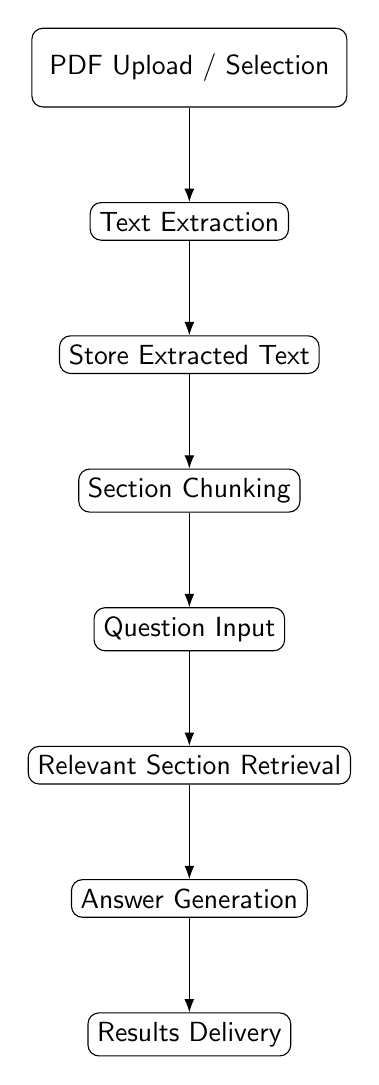
\begin{tikzpicture}[node distance=1.2cm, every node/.style={font=\sffamily}]
    \node (upload) [rectangle, draw, rounded corners, minimum width=4cm, minimum height=1cm] {PDF Upload / Selection};
    \node (extract) [rectangle, draw, rounded corners, below=of upload] {Text Extraction};
    \node (store) [rectangle, draw, rounded corners, below=of extract] {Store Extracted Text};
    \node (split) [rectangle, draw, rounded corners, below=of store] {Section Chunking};
    \node (questions) [rectangle, draw, rounded corners, below=of split] {Question Input};
    \node (retrieve) [rectangle, draw, rounded corners, below=of questions] {Relevant Section Retrieval};
    \node (answer) [rectangle, draw, rounded corners, below=of retrieve] {Answer Generation};
    \node (output) [rectangle, draw, rounded corners, below=of answer] {Results Delivery};

    \draw[-{Latex}] (upload) -- (extract);
    \draw[-{Latex}] (extract) -- (store);
    \draw[-{Latex}] (store) -- (split);
    \draw[-{Latex}] (split) -- (questions);
    \draw[-{Latex}] (questions) -- (retrieve);
    \draw[-{Latex}] (retrieve) -- (answer);
    \draw[-{Latex}] (answer) -- (output);
\end{tikzpicture}

\section{Web Application Flow}
\begin{enumerate}
    \item User navigates to the homepage.
    \item User uploads a PDF and enters one or more questions (one per line).
    \item The app checks for a stored extracted text file for the PDF.
    \item If stored text exists, the app loads it; otherwise, it extracts and stores the text.
    \item Text is split into sections and the AI reasoning flow is executed for each question.
    \item The results page displays answers, reasoning, and relevant sections for each question.
\end{enumerate}

\section{Command-Line Flow}
\begin{enumerate}
    \item User runs \texttt{python main.py}.
    \item The system loads the stored extracted text for the target PDF or extracts it if missing.
    \item The text is split into sections.
    \item The user enters questions sequentially.
    \item For each question, the system retrieves relevant sections and generates an answer.
    \item Results are printed to the terminal.
\end{enumerate}

\section{Implementation Notes}
\begin{itemize}
    \item \texttt{parser.py}: handles PDF text extraction and persistent storage of extracted text.
    \item \texttt{tree.py}: splits raw text into meaningful sections for retrieval.
    \item \texttt{reasoner.py}: selects relevant sections and generates answers using the AI backend.
    \item \texttt{app.py}: web server handling uploads and multi-question processing.
    \item \texttt{main.py}: command-line interface for sequential questions.
\end{itemize}

\section{Storage Behavior}
Extracted text is stored in \texttt{stored\_texts/} using the PDF filename as the base name. This allows repeated queries on the same PDF without re-extracting text.

\end{document}
